
\documentclass[12pt,a4paper]{article}
\usepackage[utf8]{inputenc}
\usepackage[german]{babel}
\usepackage[T1]{fontenc}
\usepackage{amsmath}
\usepackage{amsfonts}
\usepackage{amssymb}
\usepackage{graphicx}
\usepackage[left=2cm,right=4cm,top=2cm,bottom=2cm]{geometry}


\author{Steffen Specker}
\title{Unser erstes Dokument}

\date{\today}


\begin{document}

\maketitle
\tableofcontents

\newpage

\section{Einführung}

Tralalal La
\\
\\
\\
\\
Ein weiterer Test zum Mergen.
\\
\\




\subsection{Formeln}

\LaTeX{} ist auch ohne Formeln sehr nützlich und einfach zu verwenden. Grafiken etc sind kein Problem.


\begin{figure}[h]
\begin{center}
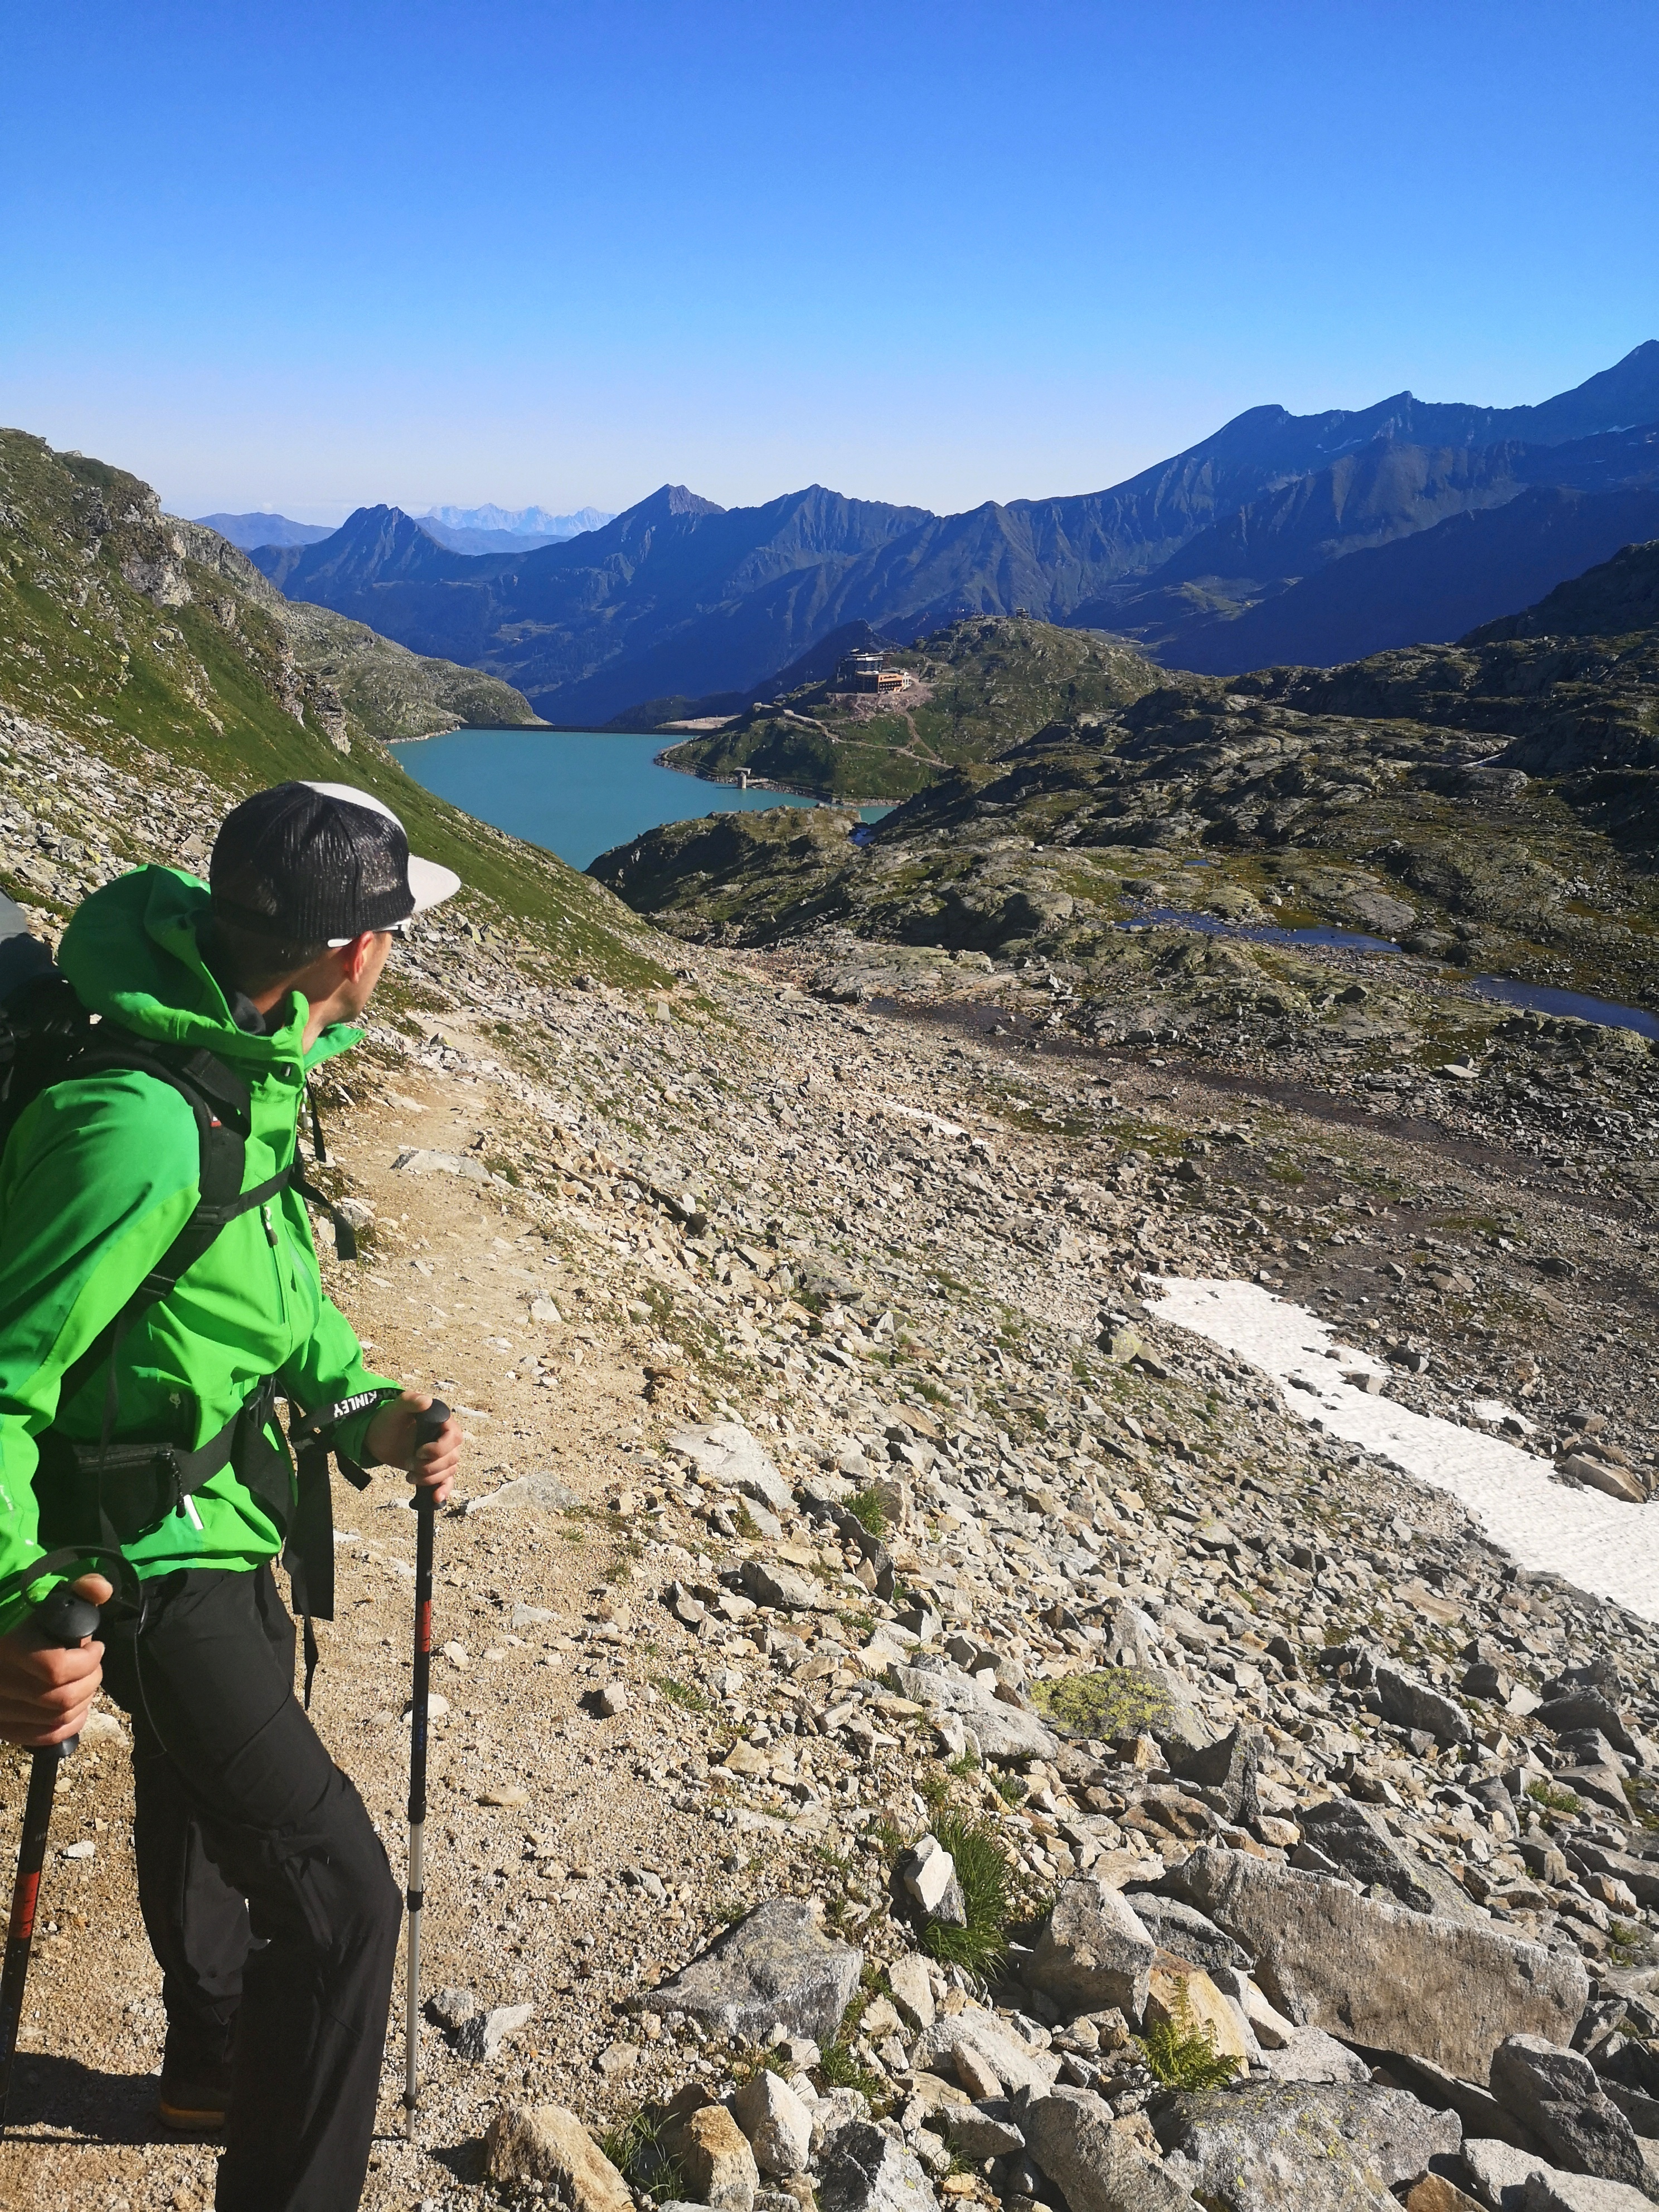
\includegraphics[width=4cm]{wandern.jpg}
\caption{Wandern in den Bergen}
\label{wandern.pgtest}

\end{center}
\end{figure}

Hallo moin test

Noch ein Test. Simon bitte einmal bestätigen.

\begin{align*}
E &= mc²
\end{align*}
Eine Erweiterung ist sehr nützlich.
Eine kleine Änderung für mich.
Noch eine Änderung.




\end{document}


